\documentclass[a4paper,11pt]{article}

\usepackage[english]{babel}
\usepackage[utf8x]{inputenc}
\usepackage{amsmath}
\usepackage{graphicx}
\usepackage{cite}
\usepackage{hyperref}
\usepackage{fullpage}
% \usepackage{apacite}
\setlength{\parskip}{1.2ex}
\begin{document}

\title{Open Information System: Conceptual schema}
\author{Thomas Perale -- 0546990\\Maximilien Romain -- 0543411\\Felipe Rojas -- 0542569\\Lehal Sherik -- 0543118}
\date{27 October 2017}

\maketitle

\section{Project subject}

Our Webowl have seven classes, Category, Ebook, Purchase, Publisher, Author, User, Publisher and Role.
User class has seven attributes which are pay information, name, email, password, userID, lastName which is connected by "hasRole" relation where the domain is the User class and the range the class Role with the attributes description and ID. Purchase class with attributes ID and Timestamp, is bounded to User class by "isMaking" relation where the User is the domain and Purchase is the range. 


Also User class is bounded to the eBook class, with its attributes year, version, title and ISBN, by the relation "hasPurchased" where the User is the domain and eBook class is the range because of the second rule, that is explained below. The eBook class will related to Purchase class through the relation “isPartOf” where the domain is the ebook class and the range is the purchase class. 
Class named Rating with attributes ID\_Rating and Number, is connected to eBook with the domain eBook and range Rating and User class with the domain User and range Rating through the relations “hasRating” and “hasRated” respectively.

The eBook class is bounded to Category class, with its attributes category\_ID and description, by the relation "hasCategory", where domain is ebook and the range is Category. Also the Category class has the relation “subCategoryOf” which infers that an eBook can have two categories, making one of them a subcategory as explained below in the rule one.

The eBook class is also bounded to the Publisher class by the relation "isPublishedby", where Ebook class is the domain and Publisher class is the range. The attributes of the Publisher class are the publisher\_ID and name. 

The Author class, has three attributes, author\_ID, first name and last name, and is bounded to Ebook class by "hasWritten" where the domain is the Author class and the range is the Ebook class. 
Rules

\section{Rules description}
First rule, if the category of a book is also a subCategory of another category, it implies that the book belongs to both category and subcategory.\\
Ebook(?x), Category(?y), Category(?z), subCategoryOf(?y, ?z), hasCategory(?x, ?y), differentFrom(?y, ?z) $\rightarrow$ hasCategory(?x, ?z)

Second rule, if an user has Purchased an ebook, and ebook is part of a purchase, then we infer that a user “HasPurchased” an ebook. \\
User(?x), Purchase(?y), Ebook(?z), isMaking(?x, ?y), isPartOf(?z, ?y) $\rightarrow$ hasPurchased(?x, ?z)

Third rule, if a user has rated an ebook and an ebook has been rating, infers that user purchased the book.\\
User(?x), Rating(?y), Ebook(?z), hasRating(?x, ?y), hasRating(?z, ?y) $\rightarrow$ hasPurchased(?x, ?z)

This last rule allows to infer that if an user has the role admin, that user can manage the ebooks on the system\\
User(?admin), Ebook(?book), AdminRole(?role), hasAdminRole(?admin, ?role) $\rightarrow$ manage(?admin, ?book)

\section{ER Schema}

\begin{center}
  \makebox[\textwidth]{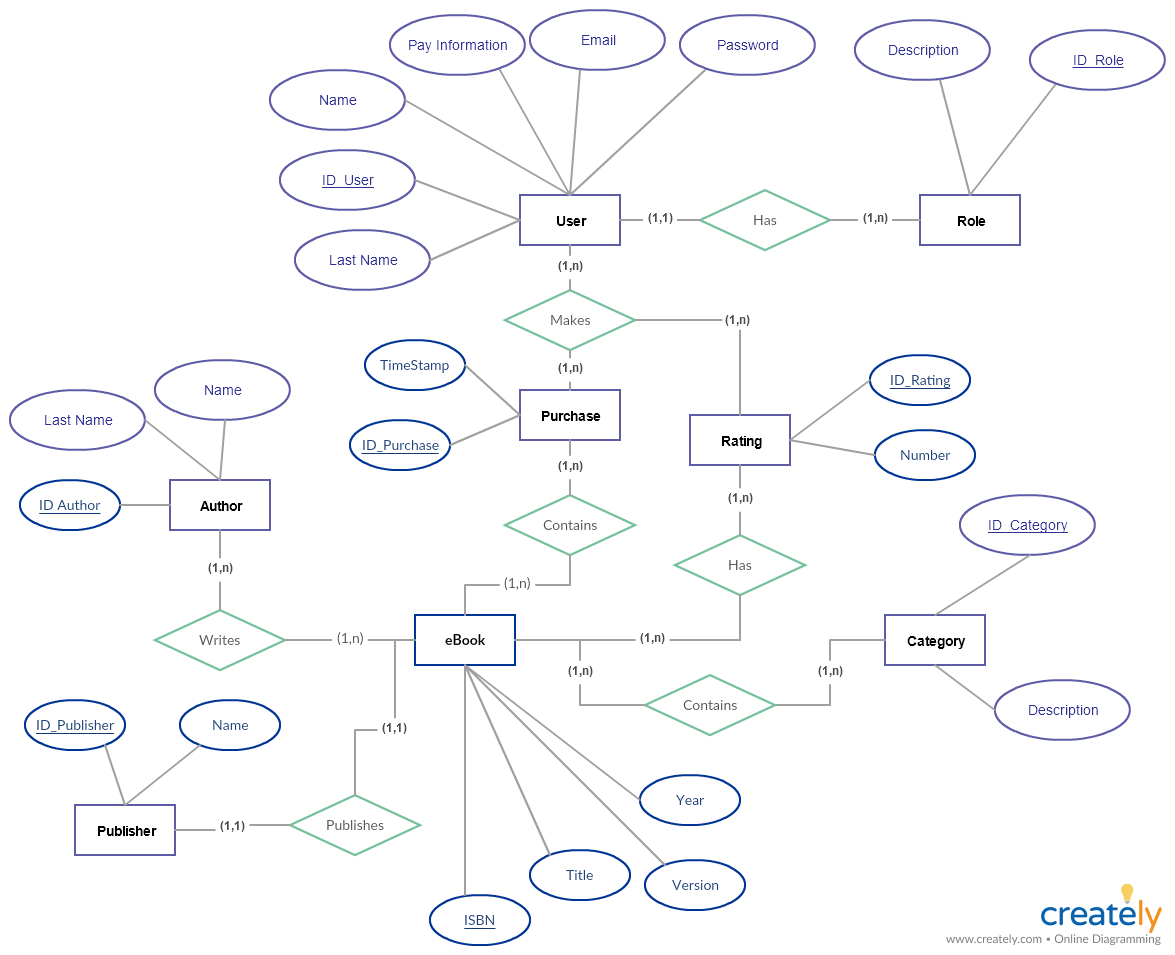
\includegraphics[width=\paperwidth]{ER_graph.png}}
\end{center}

\end{document}
